%%=========================================
\section[Metoder \& Implementasjon]{Metoder \& Implementasjon}
%%=========================================
\subsection{Min subjektivitet}
{\color{red}Fra mitt utsiktspunkt, hva har vært min interesse, hva kan jeg ha oversett, hvordan har jeg ikke vært objektiv, hvordan jeg kom inn i prosjektene med egne ideer (lineære klassifiseringsalgoritmer, kontekstdrevet brukergrensesnitt), hva jeg dermed ikke har sett nærmere på}



\subsection{Fire hypoteser}
Når hjemmet ditt om noen år tilbyr kontroll over ikke bare lys og temperatur, men garasjeporter, persienner, tv-er, radioer, låsene på døra og statusen til kjøkkenapparater, kan det være en utfordring å tilby gode interaksjonsmetoder. Løsningen på dette har hittil enten vært å la kontrollknappene være en del av apparatet eller å samle de i et panel på veggen, i en fjernkontroll eller i en app. Med et økende antall styrbare enheter blir det raskt upraktisk å kun ha kontroll dersom man fysisk befinner seg ved apparatet. Dermed kan det virke fornuftig å tilby kontroll gjennom en fjernkontroll eller en app. Men vil man alltid ha kontroll på hvor denne mobilen enheten befinner seg? I tillegg må en fjernkontroll eller app også designes godt for å unngå forvirring med et vanskelig brukergrensesnitt. Vi har alle vært uerfarne brukere av en ny fjernkontroll og opplevd større eller mindre problemer med å utøve kontroll over det aktuelle apparatet. Så kanskje det ikke er en dum idé å tilby et fast sted i rommet der kontrollen over aktuelle enheter er samlet? Det tradisjonelle panelet med knapper og dimmere er ikke bare stygt, men det er i tillegg vanskelig å vite hvilke knapper som hører til hvilken funksjonalitet (se figur \ref{fig:panel}). Det ideelle hadde kanskje vært å tilby et fast sted i rommet der kontroll kan utføres, men som er minimalistisk og allikevel kan styre et stort antall enheter. Hva hvis brukere kunne utføre enkle gester i luften foran en svært liten sensor, strategisk plassert på veggen?
\begin{figure}
\centering
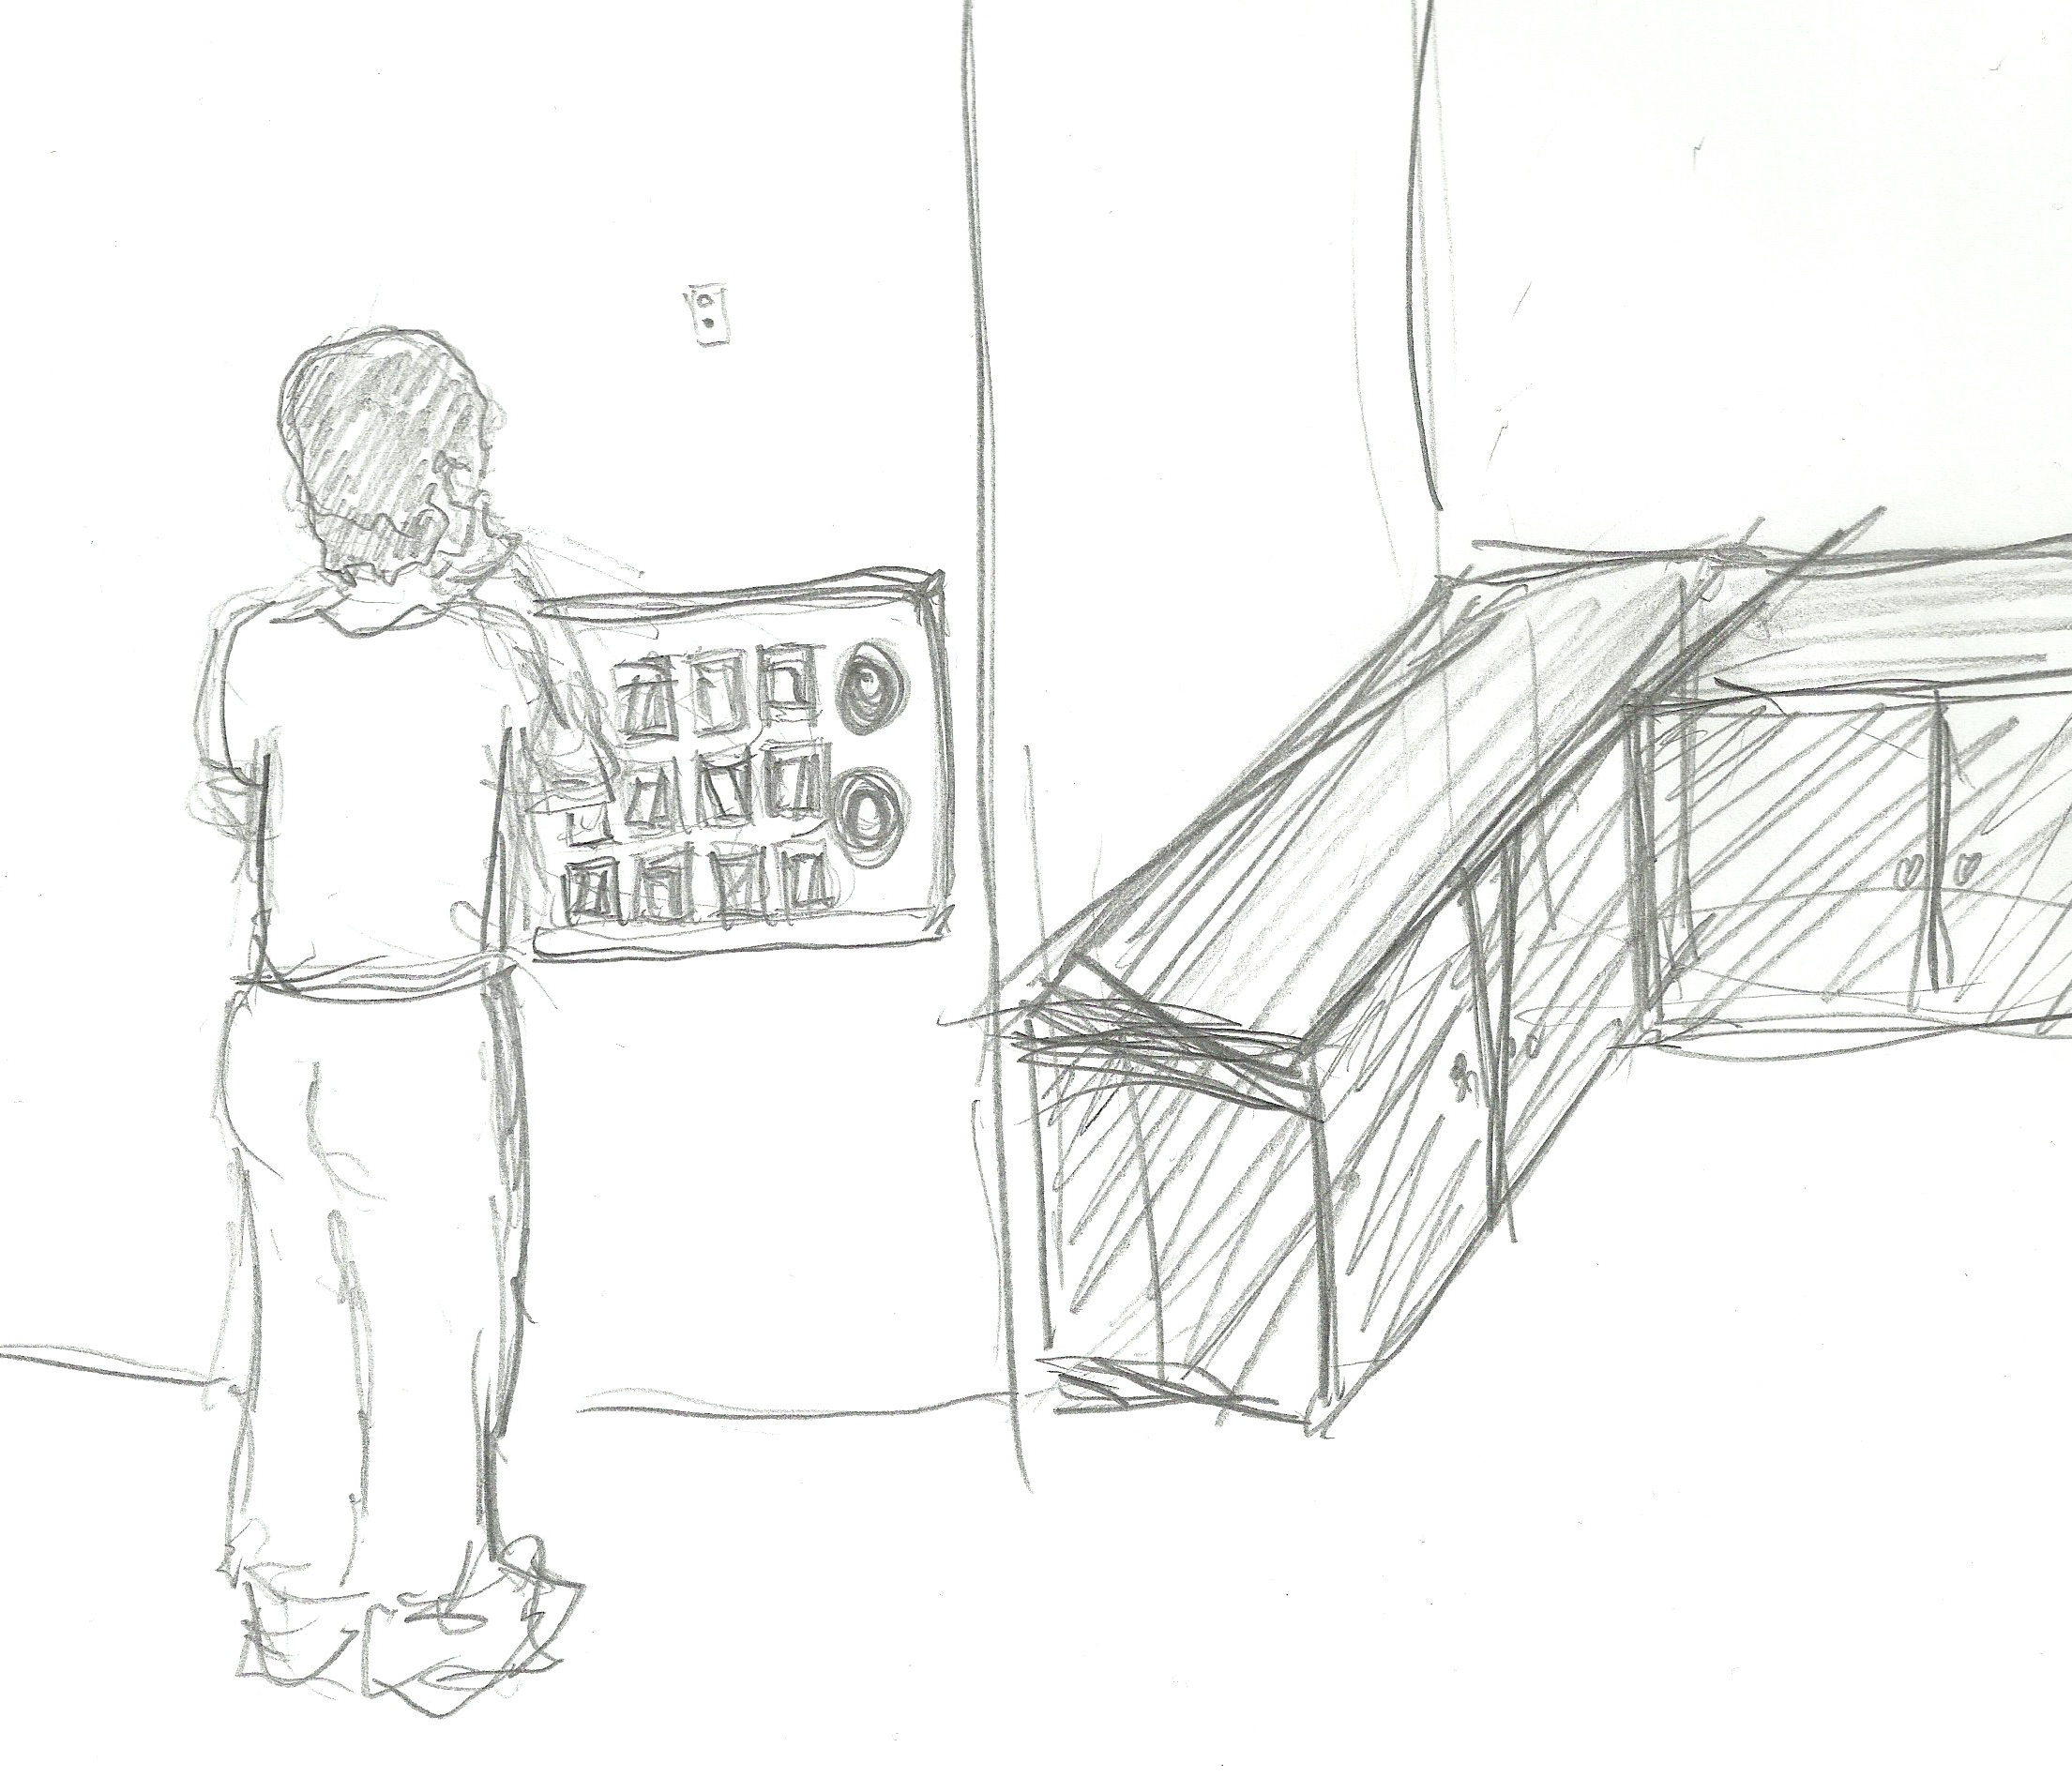
\includegraphics[scale=0.1]{fig/buttons}
\caption{En vegg med knapper skaper forvirring.}
\label{fig:panel}
\end{figure}\newline\newline
\textbf{Hypotese 1 - Gestegjenkjennelse gjennom fotodioder}\newline
\emph{En enkel sensor kan benyttes som en multifunksjonell, mekanisk bryter, og bruk av maskinlæring kan gi sensoren evnen til å skille mellom flere kommandoer enn eksplisitt programmering kan.}\newline

Programvare for å forstå tale blir stadig bedre. Desverre er det et stort problem å lage et brukbart system i scenarier der programvaren skal lytte etter kontinuerlig tale og må kunne skille mellom hva som er en kommando, og hva som kun er ordinær tale mellom mennesker. Det ville for eksempel vært et problem dersom alle som kom hjem på besøk måtte få en innføring i alle ord som ville utløse kommandoer og som de ikke kunne bruke mens de var i huset. Kommersielle systemer for talegjenkjenning løser gjerne dette ved å lytte etter et kodeord. Forståelse av naturlig språk har et annet stort problem. Den stadige forbedrede forståelsen kommer med en pris; prosesseringen og forståelsen av taledata må foregå i kraftige serverparker langt unna brukeren. Dette er et problem, både med tanke på personvern og det praktiske med at det er en ikke ubetydelig ventepause på at resultatet returneres til brukeren. Kanskje det ikke er nødvendig å forstå naturlig, kontinuerlig tale for å tilby kontroll over hjemmet? \newline\newline
\textbf{Hypotese 2 - Multimodal interaksjon gjennom tale og gester}\newline
\emph{Kombinasjonen av enkle gester og begrenset tale er en tilstrekkelig, naturlig og effektiv måte å kontrollere hjemmet på. Det er er uproblematisk å implementere et slikt system med åpen kildekode.}\newline

En gest utført foran flere sensorer i en viss konfigurasjon vil skape mer data. Det virker derfor rimelig å anta at mer data kan lede til en enda mer nøyaktig forståelse av ulike kommandoer. Sensorene har også muligheten til å måle andre verdier, som lys-nivåer, nærhet og tilstedeværelse. Kan disse egenskapene utnyttes i et smart hjem?\newline\newline
\textbf{Hypotese 3 - Kombinasjoner}\newline
\emph{Ved å benytte flere sensorer i kombinasjon kan man oppnå en høyere presisjon enn ved bruk av en enkelt sensor. Med flere sensorer kan flere kommandoer utføres naturlig av brukeren og forstås effektivt av programvaren. Sensorenes evne til å måle lys, nærhet og tilstedeværelse kan også utnyttes for å gi verdi i et smart hjem.}\newline

Standard programvare for styring av smarte hjem består av  grafiske brukergrensesnitt der metaforiske objekter, som knapper og brytere skal manipuleres. Er dette egentlig nødvendig? Brukerne bryr seg ikke om disse kunstige objektene. De bryr seg om informasjonen om hjemmet og å forstå valgene de kan ta. Den eneste modellen som skal manipuleres befinner seg i hodene deres. Et grafisk brukergrensesnitt for smarte hjem er informasjonsprogramvare og bør designes som en informasjonsgrafikk og ikke som manipulasjonsprogramvare.\newline\newline
\textbf{Hypotese 4 - Kontekstdrevet brukergrensesnitt}\newline
\emph{Et grafisk brukergrensesnitt for det smarte hjemmet bør være kontekstsensitivt og være drevet data, ikke interaksjon med brukeren.}\newline




\subsection{Design av eksperimenter}
{\color{red}Eksperimentene bør kanskje forklares i større detalj, og ikke bare som et utgangspunkt som skal utforskes? Alternativer bør foreslås og utforskes? Begrunnelse for alle valg!}
\subsubsection*{Gestegjenkjennelse gjennom fotodioder}
For å teste denne hypotesen må det først finnes fram en aktuell sensor og deretter etablere at den kan benyttes som en multifunksjonell mekanisk bryter. Med dette grunnlaget kan man forsøke å prosessere dataene sensoren lager og bygge programvare som kan lære forskjellene i dataene ulike gester produserer. Resultatene fra dette trente programmet må være tilsvarende eller bedre enn resultatene fra et eksplisitt programmert system. Det er to dimensjoner til resultatet: antall ulike gester som forstås og hvor ofte gestene forstås korrekt.

\subsubsection*{Multimodal interaksjon gjennom tale og gester}
Denne hypotesen utfordres med argumentasjon mot kontinuerlig tale i forbindelse med personvern og responstid. Videre må det argumenteres for at enkle gester og begrenset tale er akkurat det vi ønsker i forbindelse med hjemmet (programvare: kommunikasjon). Det må vises hvordan multimodal input kan håndteres, og det må vieses at åpen kildekode kan benyttes og gir tilfredsstillende resultater.

\subsubsection*{Kombinasjoner}
Her må det igjen utføres maskinlæring. Bruken av flere sensorer må gi et betydelig bedre resultat i en eller begge dimensjoner. Deretter må det kunne vises at de andre egenskapene ulike enkle sensorer har kan benyttes produktivt i forbindelse med et smart hjem.

\subsubsection*{Kontekstdrevet brukergrensesnitt}
Denne hypotesen testes ved å implementere et grafisk brukergrensesnitt og argumentere for og vise hvordan det er overlegent tradisjonelle interaksjonsdrevne systemer.





\subsection{Implementasjon}
{\color{red}Hvordan kan eksperimentet implementeres? Hvordan ble det implementert? Alle valg tatt under implementasjonen skal begrunnes, og alternativer skal ha vært utforsket!}
De følgende underkapitlene diskuterer først hvordan hvert eksperiment kan implementeres og greier så ut om hvordan jeg valgte å implementere dem.

\subsubsection{Gestegjenkjennelse gjennom fotodioder}
{\color{red}Kildekoden til dette eksperimentet representerer implementasjonen og finnes i appendix. Ref til kildekode.}
For å gjennomføre eksperimentet trengs det tilgang til en sensor som produserer tilstrekkelig detaljert data når et objekt føres i nærheten. Dataene må overføres fra sensoren til en kraftigere datamaskin. Her må dataene behandles og forberedes til maskinlæring. Til slutt trengs det gode biblioteker for læringen, gjerne med en rekke tilgjengelige algoritmer så flere tilnærminger kan forsøkes. Maskinlæringsalgoritmer er sjeldent svært avanserte og vanskelige å implementere, men for å oppnå gode resultater hurtig trengs optimaliserte implementasjoner. Det virker derfor rimelig å lete etter passende biblioteker, framfor å implementere egne algoritmer.

For å implementere eksperimentet har jeg brukt sensoren \emph{APDS-9960} fra Avago Technologies{\color{red}ref}. Denne sensoren har flere funksjoner og tilbyr måling av lys og farge, oppdagelse av nærhet og gestegjenkjennelse. Innpakningen er svært liten på kun 3.94 * 2.36 * 1.35 mm, og kan ses i figur \ref{fig:sensor-size}. Gestesensoren selv består av fire fotodioder, som kan oppfatte et infrarødt signal. En LED sender ut det infrarøde signalet og dersom et objekt befinner seg innenfor omtrent 20cm vil signalet reflekteres tilbake med nok styrke til å bli oppfattet av sensoren {\color{red}tegning?}. Fotodiodene er vinklet litt forskjellig slik at de plukker opp refleksjoner på ulike steder. Sensoren benytter resultater fra nærhetsdetektoren for å automatisk aktiveres når et objekt er innen rekkevidde. I tilegg brukes måling av lys for å tilpasse de infrarøde målingene til lysnivået i omgivelsene. Dataene dannes som 32-bit datasett og kommuniseres over I2C-protokollen til en mikrokontroller. Sensoren kan i følge fabrikanten selv håndtere forståelse av gester som passerer opp, ned, mot venstre eller mot høyre over sensoren. For å utvikle systemet er Sparkfun's innpakning av APDS-9960-sensoren benyttet. Figur \ref{fig:sensor-size} viser APDS-9960-sensoren på Sparkfun-brettet. Dette brettet gjør sensoren tilgjengelig for enklere prototyping ved å bryte ut ulike pinner. I tillegg har Sparkfun skrevet programvare til Arduino-plattformen så utviklere kommer raskt i gang og kan gjøre bruk av de forskjellige funksjonalitetene hos APDS-9960-brikken.
\begin{figure}[h]
\centering
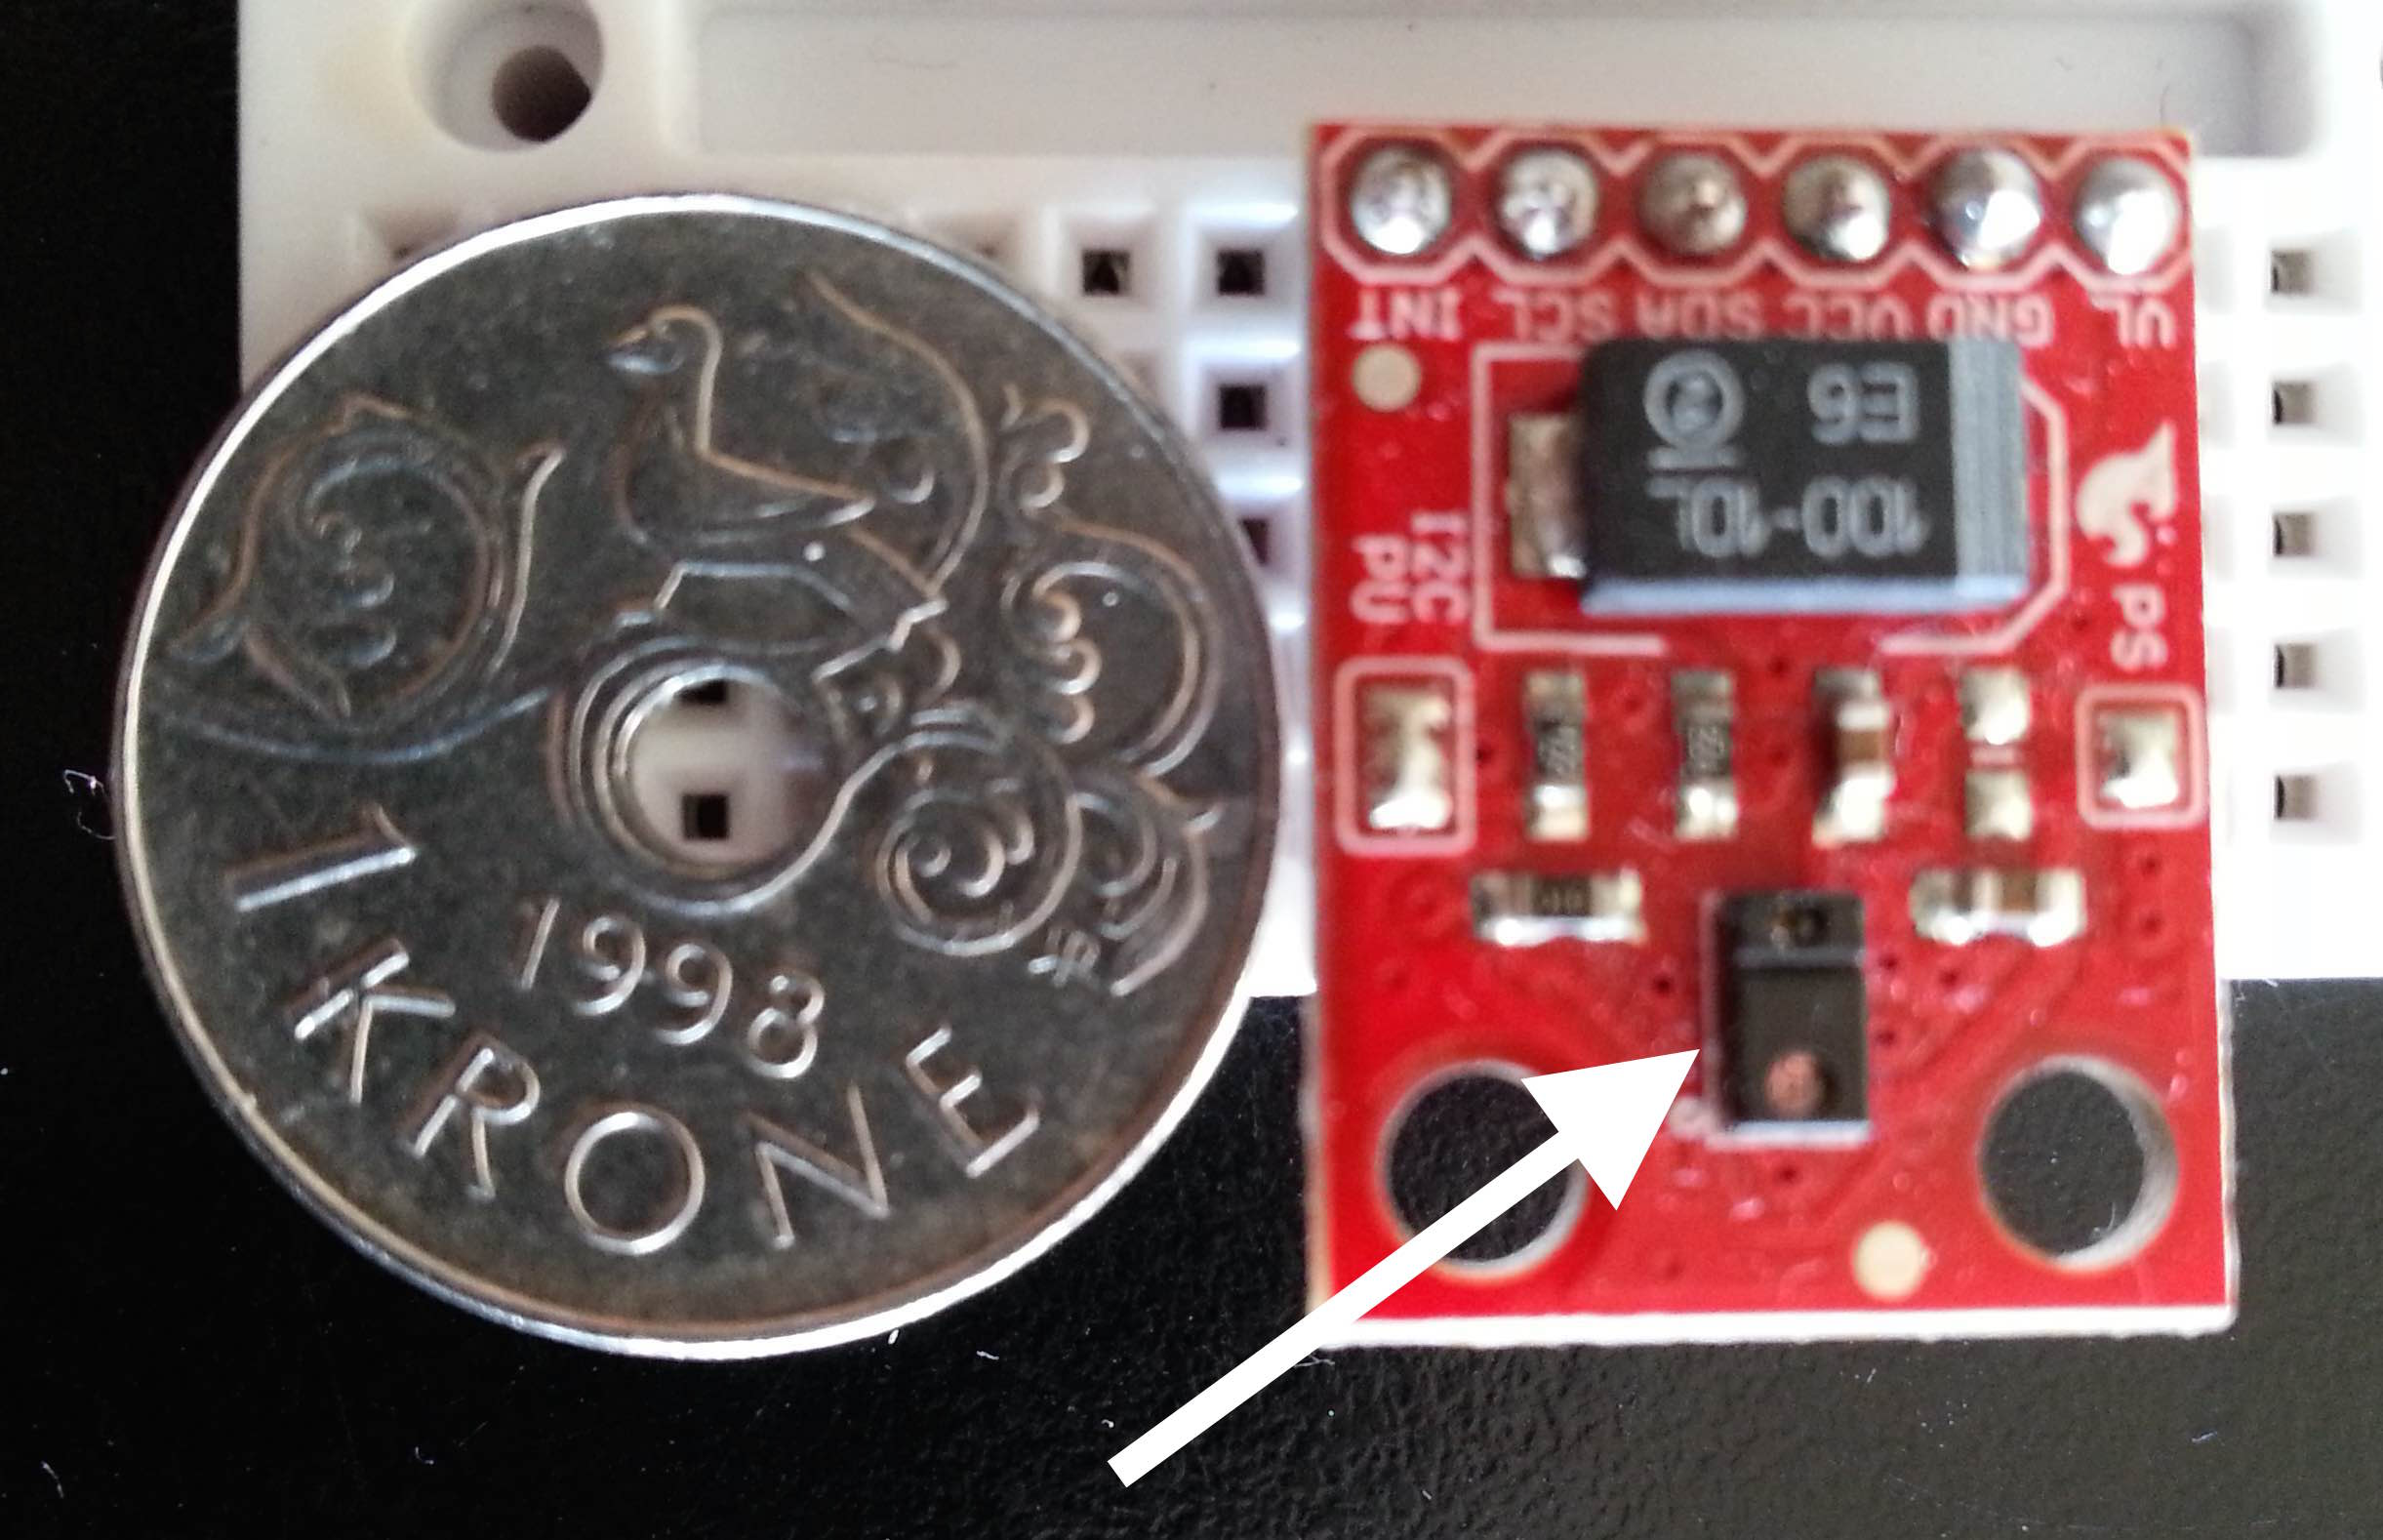
\includegraphics[width=7.5cm, height=5cm]{fig/sensor-size}
\caption{Sensorstørrelse: APDS-9960, montert på Sparkfun-brettet.}
\label{fig:sensor-size}
\end{figure}

\begin{table}[h!]
%\centering
\begin{tabular}{|| c c ||}
\hline
 Utstyr & Bruksområde \\
 \hline\hline
 Sparkfun APDS-9960 & Gestesensor \\ 
 \hline
 Level-shifter & Konverterer mellom 5V og 3.3V \\
 \hline
 Breadboard & Montere sensor og level-shifter for enklere prototyping \\ 
 \hline
 Break-away headers & Montere sensor og level-shifter til breadboard   \\ 
 \hline
 Loddebolt og tinn & Lodde headers til sensor og level-shifter\\
 \hline
 Ledninger & Overføre signal mellom sensor, level-shifter og Arduino \\
 \hline
 Arduino Uno & Drive sensoren og sende data til datamaskinen\\
 \hline
 USB-kabel & Overføre data til datamaskinen \\
 \hline
 Macbook Pro & Håndtere data og utføre maskinlæring\\
 \hline
\end{tabular}
\caption{Utstyrsliste eksperiment 1.}
\label{table:utstyrsliste}
\end{table}

For å trene systemet kreves data og for å få dataene inn til datamaskin kreves en mikrokontroller. Med Sparkfuns programvare for Arduino var det naturlig å velge en Arduino som mikrokontroller. Arduinoen ble koblet til sensoren ved å følge oppkoblingsguiden på hjemmesidene til Sparkfun {\color{red}ref}. Gestesensoren drives på 3.3V, mens en normal Arduino Uno drives på 5V. Dermed ble det nødvendig å introdusere en level-shifter, for å konvertere fra 5V til 3.3V. Figur \ref{fig:single-sensor} viser hvordan komponentene ser ut etter å ha blitt koblet sammen og er klargjort for å utføre eksperimentet. Etter at Arduinoen, sensoren og datamaskinen har fått kontakt kan jeg benytte programvaren til Arduino-plattformen til å laste opp koden som trengs for å drive sensoren. Jeg tilpasset biblioteket fra SparkFun minimalt, slik at Arduinoen ikke selv forsøker å forstå sensordataene, men i stedet sender dataene videre til datamaskinen.
\begin{figure}[h]
\centering
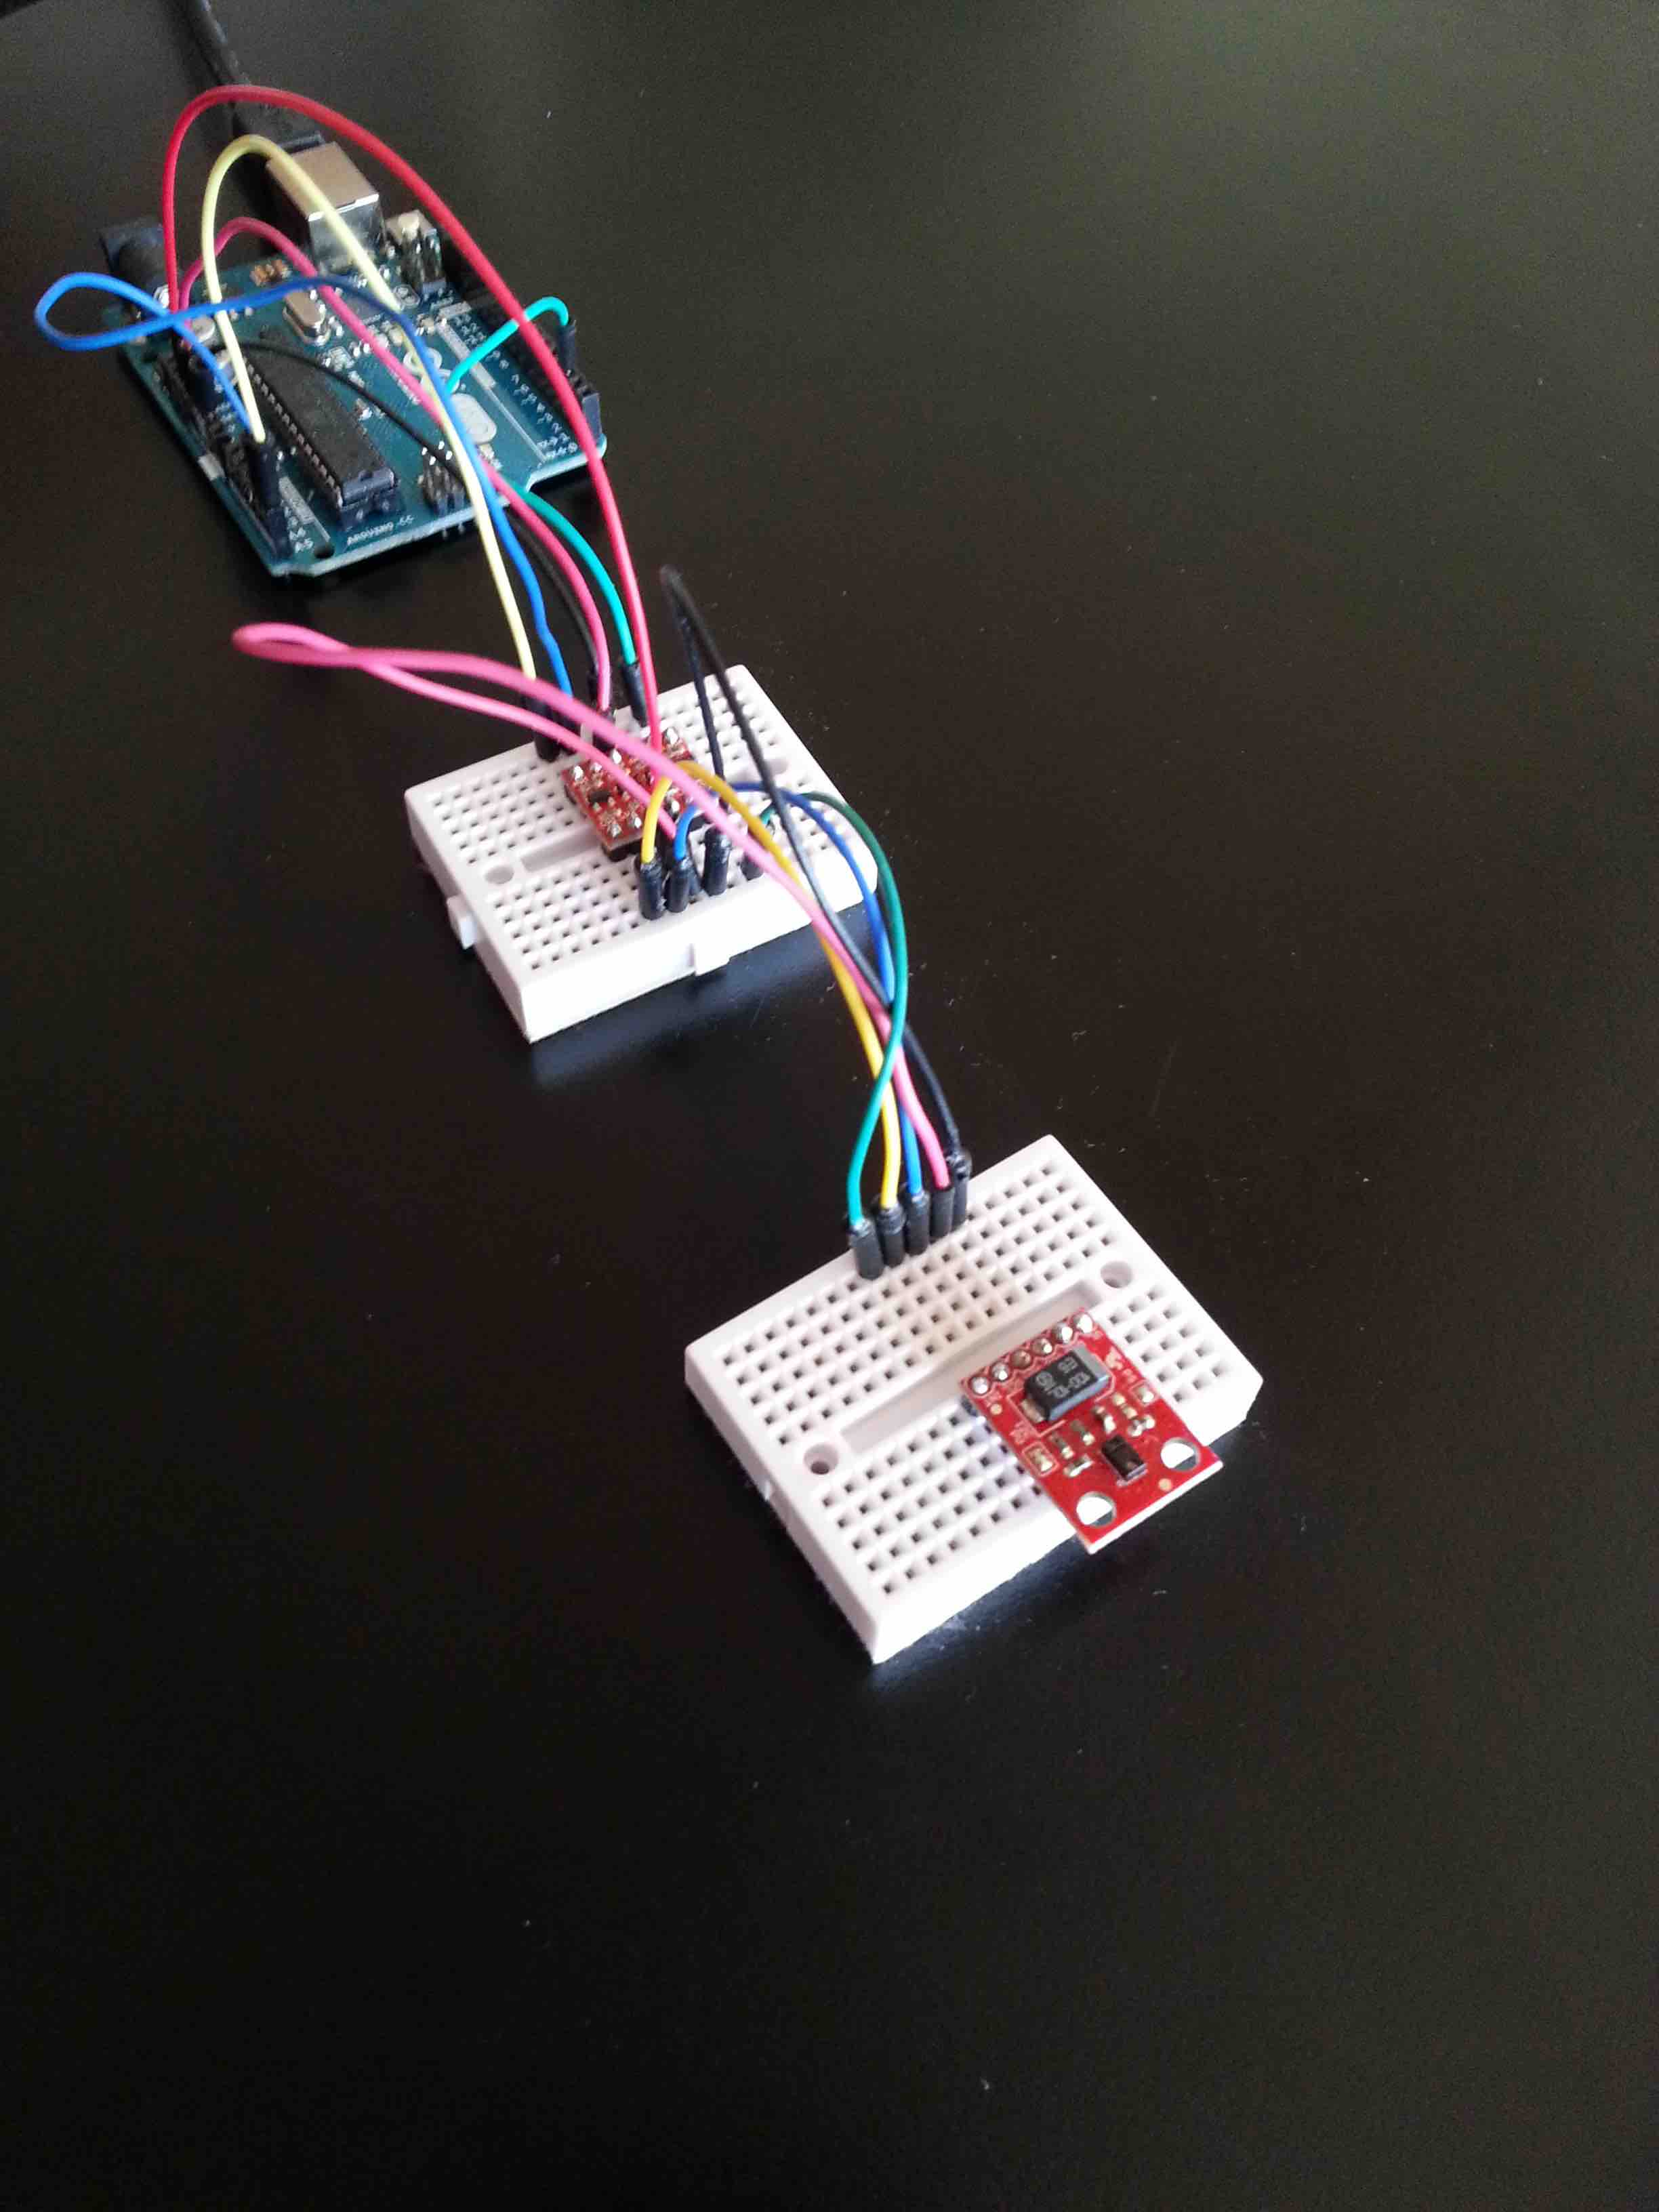
\includegraphics[width=10cm, height=10cm]{fig/singlesensor}
\caption{Sensor, level shifter og Arduino.}
\label{fig:single-sensor}
\end{figure}
For å håndtere dataprosesseringen og utføre maskinlæring valgte jeg programmeringsspråket Python. Dette valget ble tatt med utgangspunkt i at Python har et bredt utvalg biblioteker innen både seriell kommunikasjon og maskinlæring. Jeg vurderte noen alternativer og gjorde noen utforskende forsøk med å benytte Java-plattformen og et av språkene som kjører på JVM. På samme måte som Python har Java et stort miljø og mange gode biblioteker, spesielt innen maskinlæring. Desverre støtte jeg på problemer med å håndtere den serielle kommunikasjonen. Jeg antar at bruken av en virtuell maskin skaper noe mer kompleksitet rundt å kommunisere via de noe utdaterte serielle portene. Et siste alternativ jeg vurderte var å benytte programmeringspråkene Matlab eller R, som begge er populære verktøy for forskning innen kunstig intelligens. Igjen viste det seg at Python hadde et fortrinn når det gjaldt den serielle kommunikasjonen.

Arduino-programvaren henter data via I2C-protokollen fra sensoren. Den sender så dataene videre serielt til datamaskinen som lytter på den aktuelle porten. Sensoren sender data så lenge det infrarøde signalet reflekteres. Dette betyr at en gest som tar lengre tid skaper mer data. Et raskt flikk med to fingre skaper 16-32 datapunkter. Et rolig sveip over sensoren med hele hånda kan skape 100-200 datapunkter. En gest som involverer å holde hånda foran sensoren i flere sekunder skaper hundrevis av datapunkter. Den variable mengden datapunkter skaper et problem; for å benytte de planlagte klassifiseringsteknikkene må hvert av treningseksemplene må ha like mange datapunkter.

Det finnes ulike metoder for å løse dette problemet. En av de er å bestemme et øvre antall maksimale datapunkter som skal tas med. Inputeksempler som ikke har tilstrekkelig med datapunkter får lagt til 0-verdier for å oppnå den ønskede størrelsen. Å sette en slik maksgrense på datapunkter kan desverre føre til at man mister viktig data fra gester som tar lengre tid å utføre. Og for et inputeksempel fra en rask gest vil mange datapunkter være 0. Disse problemene kan påvirke effektiviteten til læringsalgoritmen. Et annet alternativ er å velge et fast antall datapunkter vært inputeksempel skal ha. Deretter knytter man inputeksempelet til denne vektoren av fast størrelse. Dersom inputdataene har få datapunkter blir den resulterende vektoren sparsom, med dataverdiene spredt jevnt utover og med 0-verdier i mellom. Dersom inputdataene består av mange datapunkter vil hvert datapunkt i vektoren være et gjennomsnitt av en valgt mengde datapunkter.

Jeg valgte å benytte denne sistnevnte teknikken og lagde vektorer med 128 datapunkter. Dette tallet ble valgt basert på antall datapunkter som genereres ved ulike aktuelle gester. 128 datapunkter er nok til å gi tilstrekkelig detaljer selv ved gester som tar noe lengre tid og samtidig ikke så mange at raske gester skaper i overkant sparsomme vektorer. Vektoren normaliseres ved å knytte de mulige sensorverdiene [0,255] til [0,1.0]. Å illustrere dannelsen av vektorer med 128 datapunkter blir tungvint så i figur \ref{fig:data} har jeg illustrert prosessen med langt mindre data. I \ref{fig:few} består inputvektoren av to datapunkter. La oss si vi ønsker en vektor med størrelse fire og som er normalisert til verdiområdet [0,10.0]. Dette oppnås ved å spre inputdataene jevnt i vektoren og normalisere verdiene. \ref{fig:many} viser det motsatte tilfellet, der inputvektoren er for stor. For å representere dataene i en mindre vektor blir det tatt gjennomsnittsverdier som deretter normaliseres. {\color{red}Flere detaljer fra koden / vise kode?}
\begin{figure}[h]
\centering
\begin{subfigure}{0.23\textwidth}
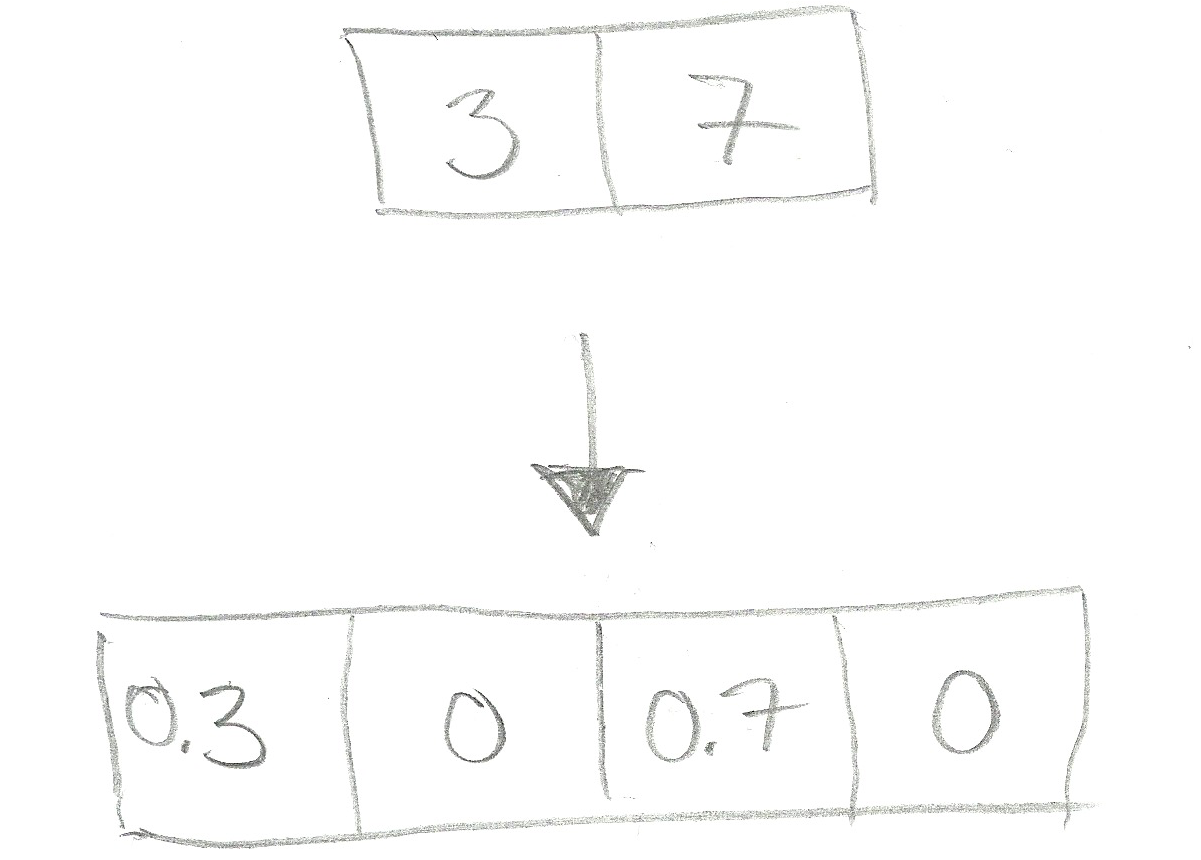
\includegraphics[width=3cm, height=3cm]{fig/few-to-many}
\caption{}
\label{fig:few}
\end{subfigure}
\begin{subfigure}{0.23\textwidth}
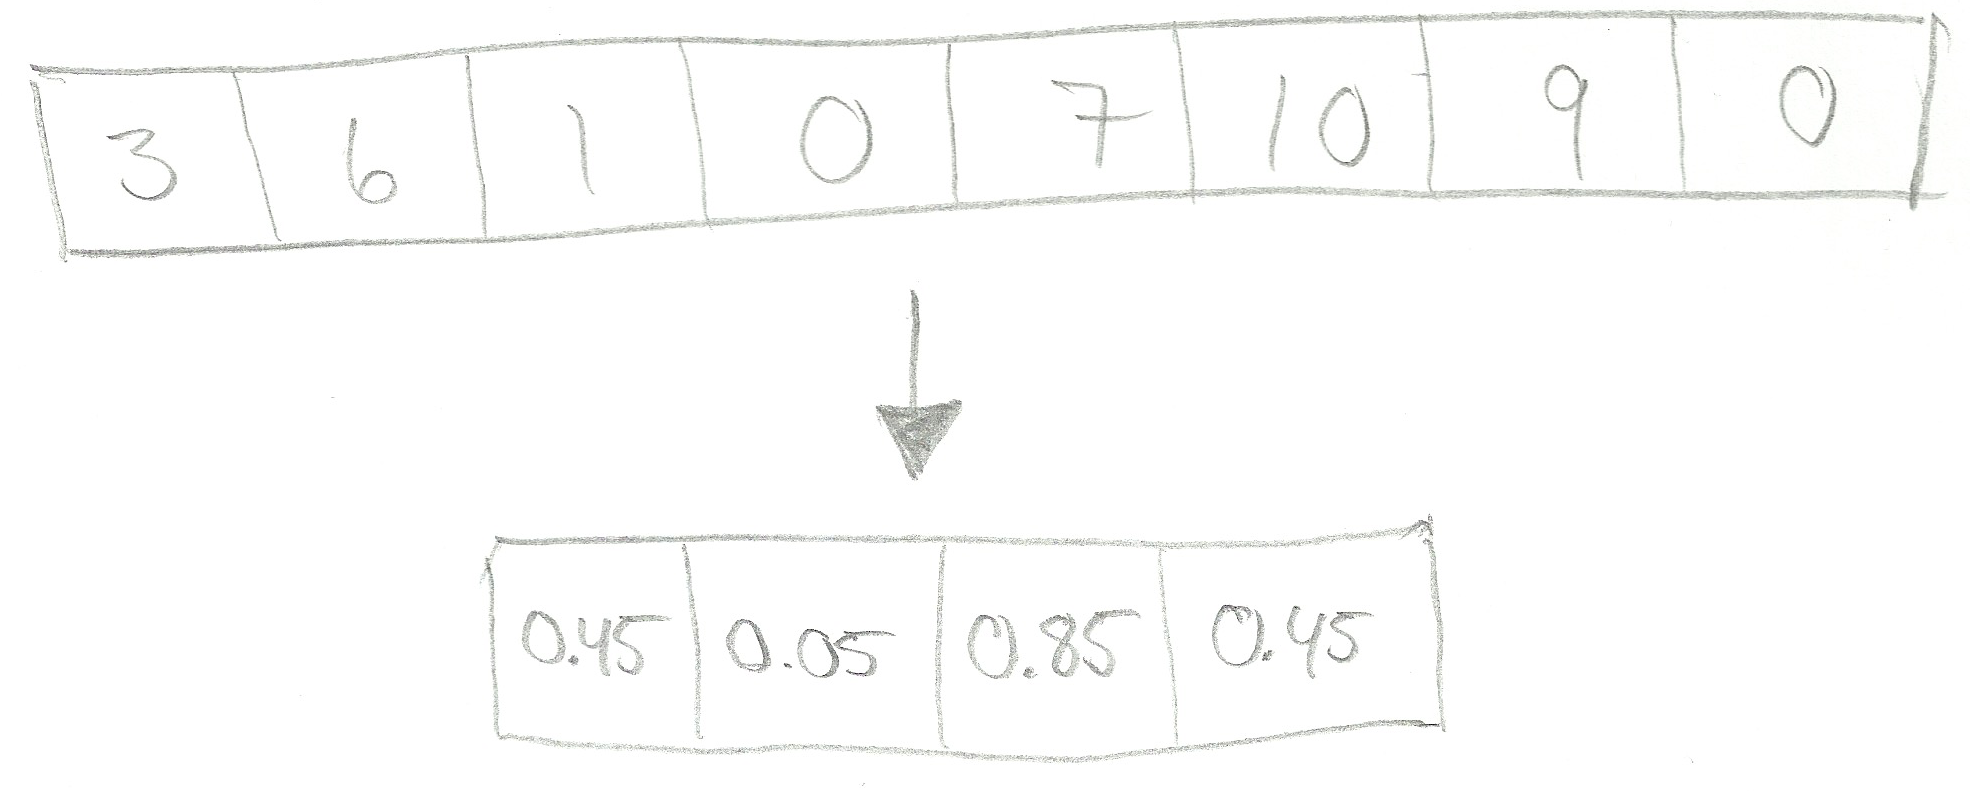
\includegraphics[width=3cm, height=3cm]{fig/many-to-few}
\caption{}
\label{fig:many}
\end{subfigure}
\caption{Illustrasjon av dannelsen av en datavektorer.}
\label{fig:data}
\end{figure}
Eksperimentet vil ha to deler. Den første delen blir å utføre en rekke eksempler på gester og lagre de prosesserte dataene. Del to er laste inn dataene i en modell kan trenes, testes og evalueres.  

For å utføre maskinlæringen benyttet jeg to Python-biblioteker: numpy og scikit-learn. Numpy er det absolutt vanligste biblioteket for numeriske kalkulasjoner i Python. For maskinlæringen finnes det mange alternativer. Scikit-learn tilbyr mange algoritmer, og er spesielt gode på de lineære klassifiseringsalgoritmene. For å benytte klassifiseringsalgoritmene scikit-learn har tilgjengelig trengs det to numpy-datasett: et datasett med dataene fra gestene, og et tilsvarende med tilhørende etiketter.

\subsubsection{Multimodal interaksjon gjennom tale og gester}
{\color{red}Hvordan kan eksperimentet implementeres? Hvordan valgte jeg å implementere det? Kode.}

{\color{red}Hvordan kan eksperimentet implementeres?}
Dersom eksperiment 1 er utført er gestegjenkjennelse tilgjengelig. Et system for talegjenkjenning må finnes eller implementeres fra bunn av. Det trengs i tillegg til utstyret fra eksperiment 1 en mikrofon.

{\color{red}Gester}
Dersom eksperiment 1 var en suksess kunne maskinlærte gester blitt brukt i kombinasjon med tale i dette eksperimentet. Men for å i utgangspunktet minimere kompleksiteten valgte jeg i dette eksperimentet å benytte Sparkfuns programvare for gestegjenkjennelse. Dette betydde at gestesensoren forstår seks ulike gester. Kombinasjonen av maskinlærte gester og tale utforskes i eksperiment 3.

{\color{red}Talegjenkjenningsprogramvare}
Det finnes alternativer dersom man ønsker å utforske programvare for talegjenkjenning. Google tilbyr sitt tale-API, men da mitt poeng er at disse tjenestene ikke er det vi ønsker i hjemmet må vi ty til andre midler. CMUSphinx er et pågående prosjekt fra Carnegie Mellom University med fri kildekode.

norsk vs engelsk

sphinx vs pocketsphinx

lage språkmodell

Etter at pocketsphinx er installert kan det startes fra kommandolinjen med:
\verb|pocketsphinx_continuous -inmic yes -lm ..sti/til/språkmodell -dict ..sti/til/ordbok|

{\color{red}Håndtering av multimodal input: køer og tråder. Hvor mye kode skal jeg ha med?}
Prat om hvor bra køer og tråder er..

\begin{lstlisting}[language=Python, caption=Kode Python bakgrunnstråd]
from threading import Thread

def start_thread(fn, args):
    worker = Thread(target=fn, args=args)
    worker.setDaemon(True)
    worker.start()
\end{lstlisting}

\begin{lstlisting}[language=Python, caption=Geste-data]
from serial import Serial

def gesture_recognition(q):
    ser = Serial('/dev/cu.usbmodem1431', 9600)
    buf = []
    while True:
        c = ser.read()
        if c == '\n':
            result = ''.join(buf)
            print(result)
            q.put(('gesture', result), block=True, timeout=1)
            buf = []
        elif c == '\r':
            pass
        else:
            buf.append(c)
\end{lstlisting}

\begin{lstlisting}[language=Python, caption=Talegjenkjenning]

\end{lstlisting}

\begin{lstlisting}[language=Python, caption=Kode Python starte trådene]
start_thread(speech_recognition, (animation_q,))
start_thread(gesture_recognition, (animation_q,))
\end{lstlisting}

\begin{lstlisting}[language=Python, caption=Kode Python multimodal]
import pyprocessing as p

def simple_multi_modal():
    source, text = animation_q.get_nowait()
    # non-blocking check for items in animation_q.
    # If queue is empty a Queue.Empty exception is raised.
    # data read from queue is a tuple of strings: (source, text)
    if source == 'gesture':
        p.fill(0, 102, randint(50,150))
        p.textSize(48)
    elif source == 'speech':
        p.fill(102, randint(50,150), 0)
        p.textSize(32)
    else:
        pass
    p.text(text, randint(50,550), randint(50,550))
\end{lstlisting}



\subsubsection{Kombinasjoner}
{\color{red}Hvordan kan eksperimentet implementeres? Hvordan ble det implementert? Kode.}

Bruksområder i smarte hjem for den andre funksjonaliteten i sensorene.
PING: Data om farger, lysintensitet, avstand og en kombinasjon av flere gestesensorer utforskes for å finne nye interaksjonsideér.
Gester
Lysstyrke / Farger kontinuerlig
Lys interrupt
Nærhetsmåling kontinuerlig
Nærhetsinterrupt
Hva kan man få til dersom man har fire sensorer plassert i et kvadrat?

\subsubsection{Kontekstdrevet brukergrensesnitt}
{\color{red}Hvordan kan eksperimentet implementeres? Hvordan ble det implementert? Kode.}

Denne fjerde hypotesen omhandler informasjonsprogramvare; hvordan relevant informasjon om hjemmet kan presenteres for brukeren.

Som regel når en person bruker programvare er det ikke for å skape noe, men for å lese, observere, utforske og lære. Folk er ute etter å ordne egne tanker. Datamaskinen er et medium for å spørre spørsmål, gjøre sammenligninger og dra konklusjoner. Det aller meste av programvare er altså \emph{informasjonsprogramvare}. 

